\section{Startups}

%%%%%%%%%%%%%%%%%%%%%%%%%%%%%%%%%%%%%%%%%%%%%%%%%%%%%%%%%%%%%%%%%%%%%%%%%%%%%%%%%%%%%%%%%%%%%%%%
\subsection{\textbf{Nos preguntamos:} ¿Qué viene a tu mente cuando piensas en startups?}
\begin{enumerate}
    \item Inicial un negocio 
    \item Alto crecimiento (ingresos)
    \item Baja disponibilidad 
    \item Alto riesgo 
    \item Empresa primitiva (a un nivel básico o inicial)
\end{enumerate}


%%%%%%%%%%%%%%%%%%%%%%%%%%%%%%%%%%%%%%%%%%%%%%%%%%%%%%%%%%%%%%%%%%%%%%%%%%%%%%%%%%%%%%%%%%%%%%%%
\subsection{Ciclo de vida de empresas}

%%%%%%%%%%%%%%%%%%%%%%%%%%%%%%%%%%%%%%%%%%%%%%%%%%%%%%%%%%%%%%%%%%%%%%%%%%%%%%%%%%%%%%%%%%%%%%%%
\subsubsection{Requisitos e información preliminar}
\begin{itemize}
    \item La capacidad de movernos a través de esa curva depende de nuestras capacidades gerenciales y empresariales.
    \item 
\end{itemize}

%%%%%%%%%%%%%%%%%%%%%%%%%%%%%%%%%%%%%%%%%%%%%%%%%%%%%%%%%%%%%%%%%%%%%%%%%%%%%%%%%%%%%%%%%%%%%%%%
\subsection{Roles de liderazgo por etapas}
\begin{itemize}
    \item Emprendedor: ejerce la función empresarial: 
        \begin{itemize}
            \item Tener en cuenta el \textbf{riesgo}, elegir las opciones y el costo de oportunidad.
            \item Navegan en caminos de alta incertidumbre.
            \item Es totalmentenovedoso o nuevo, son los primeros en introducir su producto, esto $\rightarrow$ que no hay nadie de quien se pueda aprender todo es un experimento.
        \end{itemize}

    \item Administrador: 
        \begin{itemize}
            \item Planeación, estrategia, sistema, ejecución, liderar equipos, sostenibilidad.
            \item Énfasis en \textbf{habilidades gerenciales}.
        \end{itemize}

    \item Innovador:
        \begin{itemize}
            \item Empatía, visión, disruptivo, creativo, decisivo.
            \item La innovación lo impregna todo, desde el servicio hasta el producto en sí.
        \end{itemize}
    
    \item Conciliador:
        \begin{itemize}
            \item Negociación, sinergia, empatía, creatividad.
            \item Poder aprender del fracaso, ``de todas las experiencias derivan un aprendizaje'', ``cuando un proyecto no te funcionó no es asunto de pérdida si no de aprendizaje''.
            \item \textbf{Nos preguntamos:} ¿Cuán receptiva es nuestra habilidad de aceptar nuestro fracaso?
            \item \emph{Citación:``falla amenudo para tener éxito más seguido"}.
        \end{itemize}
\end{itemize}

%%%%%%%%%%%%%%%%%%%%%%%%%%%%%%%%%%%%%%%%%%%%%%%%%%%%%%%%%%%%%%%%%%%%%%%%%%%%%%%%%%%%%%%%%%%%%%%%
\subsection{Cómo nos movemos en nuestra curva empresarial}
\begin{itemize}
    \item Evidentemente se necesita una financiación periódica, entonces \emph{la habilidad de atraer recursos}.
    \item \emph{\textbf{Ejemplo: }Alguien es muy bueno en todo, pero no es está consiente de que hay ciertas actividades que no se pueden delegar.}
    \item \textbf{Nos preguntamos:} ¿Cuáles son las fuentes de financiamiento que periódicamente necesito para crecer?
    \item Curva Bell:
        \begin{figure}[htbp]
            \centering
            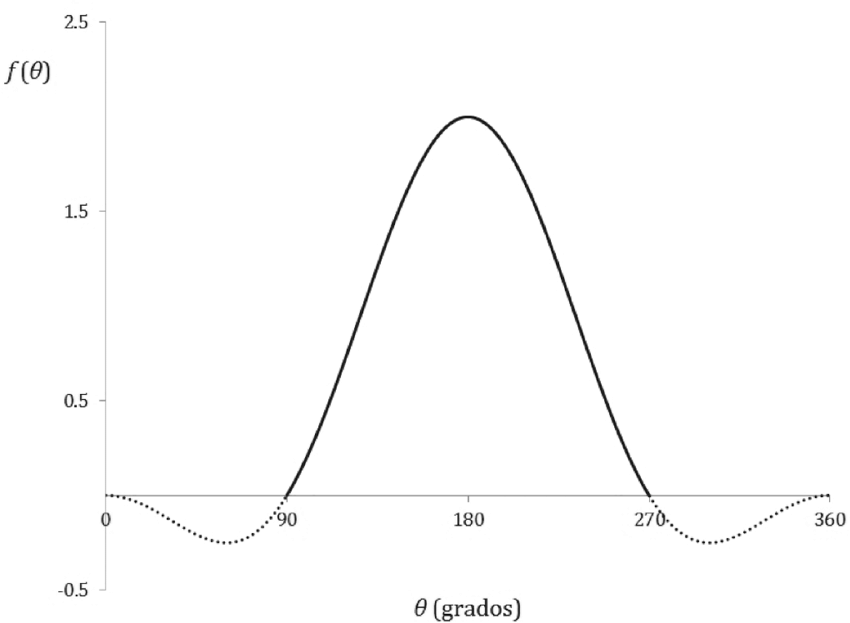
\includegraphics[width=9cm]{./../__Imagenes__/2020-02-05-Global-01.png}
            \caption{Curva de Bell}
            \label{}
        \end{figure}
        Las personas que me apoyan en este proceso: 
        \begin{enumerate}
            \item Tempraneros \emph{Early adopted}: personas dispuestas a arriesgar su dinero en cambio por apoyar a los nuevos startups, los \emph{primeros clientes leales}. 
            \item Seguidor: Las personas qu esperan a ver qué tal sale el nuevo producto innovador para evaluar si lo compra o no.
            \item Tardíos: Usualmente los que compran ek producto usado, no se ven afectados por los productos innovadores. 
        \end{enumerate}
    
    \item Crowd funding: son personas que donan,o ayudan al startup a cambio de un return incierto o nulo.
\end{itemize}


%%%%%%%%%%%%%%%%%%%%%%%%%%%%%%%%%%%%%%%%%%%%%%%%%%%%%%%%%%%%%%%%%%%%%%%%%%%%%%%%%%%%%%%%%%%%%%%%
\subsection{Ciclo de vda de la empresa}
\begin{enumerate}
    \item Riesgo alto: 
        \begin{itemize}
             \item Semilla
            \item Temprano
        \end{itemize}
    
    \item Riesgo medio:
        \begin{itemize}
            \item Medio
            \item Expansión
        \end{itemize}
        
    \item Riesgo alto: 
        \begin{itemize}
            \item Madurez
        \end{itemize}
\end{enumerate}




%%%%%%%%%%%%%%%%%%%%%%%%%%%%%%%%%%%%%%%%%%%%%%%%%%%%%%%%%%%%%%%%%%%%%%%%%%%%%%%%%%%%%%%%%%%%%%%%
\section{¿Start-ups?}
\begin{itemize}
    \item Tienen una capacidad muy efectiva a responder a nuevas tendencias sin pasar por la burocracia de las empresas grandes.
    \item El acceso a capital es carísimo, la gente está dispuesta a dar plata pero sólo si compran grandes porcentajes de la compañía.
    \item Startups:
        \begin{center}
            \begin{tikzpicture}[node distance = 2.5cm, auto, centered]
                \node [block] (1) {Steak Holder}; 
                \node [block,below of=1] (2) {Clientes}; 
                \node [block, right of=2] (3) {Proveedores};
                \node [block, right of=3] (4) {Inversionistas \$ - conocimiento};
                \node [block,left of=2] (5) {Incentivos públicos, el gobierno te ayuda}; 
                \node [block, left of=5] (6) {Comunidad, asociaciones/cámaras, para emprendedores};   
                \path [line] (1) -- (2);
                \path [line] (1) -- (3);
                \path [line] (1) -- (4);
                \path [line] (1) -- (5);
                \path [line] (1) -- (6);
            \end{tikzpicture}
        \end{center}
    
    \item La modalidad del entreprenour:
        \begin{itemize}
            \item Emprenden desde adentro.
            \item Pueden ocurrir startups \textbf{dentro de las compañías}.
        \end{itemize}
    
    \item Procesos simples:
        \begin{itemize}
            \item B2B: Business to business: 
            \item B2C: Business to consumers: 
        \end{itemize}
        Reducen intermediarios, eliminando los costos de transacción, publicidad, comisión.
    
    \item Importante usar TIC, Tecnología de Información \& Comunicación.

    \item Escalable mercadeo digital:
        \begin{itemize}
            \item \emph{\textbf{Ejemplo: }La estadística de ``internet users'' en varios países. } 
            \item Ayudan a entender el target.
            \item El propósito de el mercadeo escalable es poder llegar a la mayor cantidad de gente que pertenezca al target.
        \end{itemize}
    
    \item Start soon, easy going, plug and play, free of cheap.
        \begin{itemize}
            \item Reducir las dependencias.
        \end{itemize}
    
    \item Falla a menudo para tener éxito más seguido:
        \begin{itemize}
            \item Si sos perfecto alguien más va a lanzar un que no sea perfecto pero lanzado y ganando dinero ya.
            \item Error: ``Los emprendedores se enamoran de su producto y no validan las necesidades de los demás''.
            \item Obtén información de los clientes más amenudo así se puede mejorar el producto periódicamente.
            \item Hacer el MVP (minimum viable product).
            \item Debe de ser \textbf{Rápido, barato, sucios (borradores)}, todas las grandes empresas sacan como primera versión los MVP.
            \item Esto permite el feedback efectiva. 
            \item Adquirir feedback con los \textbf{focus groups}.
        \end{itemize}
    
    \item Autodidacta:
        \begin{itemize}
            \item Equipos multidisciplinarios de alta especialización profesionalismo.
            \item Tener recursos como videos, investigaciones, en las que me pueda ayudar a ser coaches.
            \item \emph{Citación:``no estoy esperando a que un maestro me diga qu hacer, yo soy autodidacta"}.
            \item No tienes que aprender un proceso formal de aprendizaje para poder educarse. 
            \item Gestión de tiempo es importante.
        \end{itemize}
    
    \item Star-ups - Retos: 
        \begin{itemize}
            \item \emph{Citación:``Sólo un emprendedor se sale de un trabajo para trabajar 80h"}.
        \end{itemize}
\end{itemize}


